\documentclass[10pt]{report}            % Report class in 11 points
\usepackage{mathtools}
\usepackage{amssymb,amsmath}
\usepackage{graphicx}
\parindent0pt  \parskip10pt             % make block paragraphs
\raggedright                            % do not right-justify
\title{\bf CSCI576 Assignment 1 Report}  % Supply information

\author{Hengyue Liu\\USC ID: 4107-2966-75}              %   for the title page.
\date{\today}                           %   Use current date.

\begin{document}                        % End of preamble, start of text.
\maketitle                              % Print title page.
\pagenumbering{roman}                   % roman page number for toc
\setcounter{page}{2}                    % make it start with "ii"
%\tableofcontents                        % Print table of contents
\renewcommand{\chaptername}{Part}
%\renewcommand{\thechapter}{\Alph{chapter}}
\chapter{Written Questions}                % Print a "chapter" heading
\pagenumbering{arabic}                  % Start text with arabic 1
Most of this example applies to \texttt{article} and \texttt{book} classes
as well as to \texttt{report} class. In \texttt{article} class, however,
the default position for the title information is at the top of
the first text page rather than on a separate page. Also, it is
not usual to request a table of contents with \texttt{article} class.
 
\section*{Q 1}                  % Print a "section" heading
Solutions:
\begin{itemize}
\item                           % The following text will be \begin{quote}
 $N_{l}=450$\\                                %    set off and indented.
 $N_{p}=520$\\
 $N_{FPS}=25$\\ 
 P=12 bits per pixel for 4:2:0 scheme\\
 $N_l \cdot N_p \cdot N_{FPS} \cdot P = 7.02\times10^7$ bits/s.\\
 So, the bit-rate produced by the camera is $7.02\times10^7$ bits/s.\\
\item
$4 \times 8 + 6 + 6 = 44$ bits per 4 pixels.\\
So $P'=11$ bits per pixel.\\
The bit-rate of the re-quantized signal will be $N_l \cdot N_p \cdot N_{FPS} \cdot P'= 6.435\times10^7$ bits/s. 10 minutes video will contain $6.435 \times10^7 \times 10 \times 60 \div 8 \div 1024 \div 1024 \div 1024 \approx 4.49$ GB.\\
So at least 4.5 GB storage for the disk to store the video.\\
                             % End of indented text
 \end{itemize}   
But note that---unlike the \texttt{book} and \texttt{report} classes---the
\texttt{article} class does not have a ``chapter" command.
 \section*{Q 2}                  % Print a "section" heading
 Solutions:
 \begin{itemize}
 	\item
 	Use these quantization intervals [-4, -3.625), [-3.625, -3.375) ... [3.875, 4], if the value is just in the middle of quantization levels then round it to the upper boundary level. Then the quantized sequence is:\\
 
 	[1.875, 2.125, 2.125, 3.125, 3.375, 2.625, 2.875, 2.875, 2.875, 1.625, 1.125, 1,125, 1.125, 1.875, 2.125, 2.125, 2.125, 1.875, 2.375, 1.125, 0.125, -1.125, -1.125, -1.625, -1.125, -2.125, -1.375, -1.375, -0.625, 0.125, 0.875]
 	\item
 	There are 33 levels, so it needs at least 6 bits to represent one sample. Totally $6\times32=192$ bits are needed.
 \end{itemize}
  \section*{Q 3}                  % Print a "section" heading
  Solutions:
  \begin{itemize}
  	\item
  	First calculate the perimeter of the wheel, $\pi\times0.4244 =1.3333$, then $36\times1000\div1.3333\div3600=7.5$ rotations/s, the frame rate 24 fps is larger than twice of this rotation speed, so the true speed is observed as 7.5 rotations/s.
  	\item
  	8 fps will cause aliasing,and the aliasing frequency will be $8-7.5=0.5$ rotations/s counter-clockwise.
  \end{itemize}
\chapter*{Programming Analysis Questions}
  \section*{Q 1}
  The distortion curve is generated by the average error percentage for each pixel compared to the original image.
  \begin{itemize}
  
  \item
  Distortion cure with Y varying, set U and V to 1:\\
  -0.176407  inf -0.150256
  -0.165809  inf -0.133801
  -0.173324  inf -0.0869003
  -0.179565  inf -0.00607022
  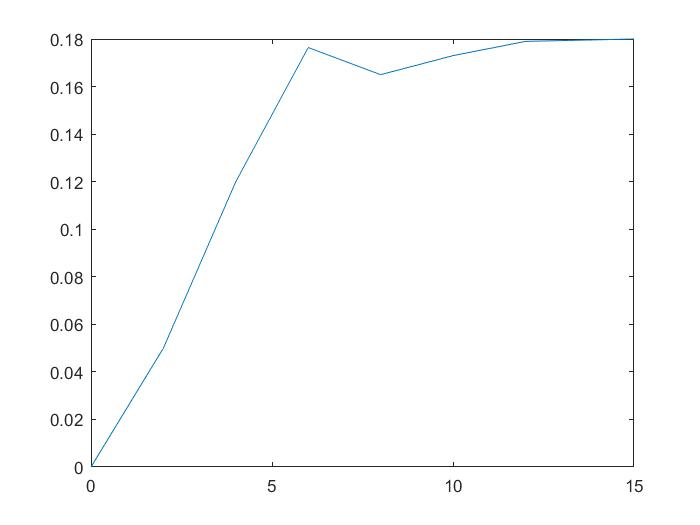
\includegraphics[height=200pt]{1.jpg}
  \item
  Distortion cure with U varying, set Y and V to 1:
  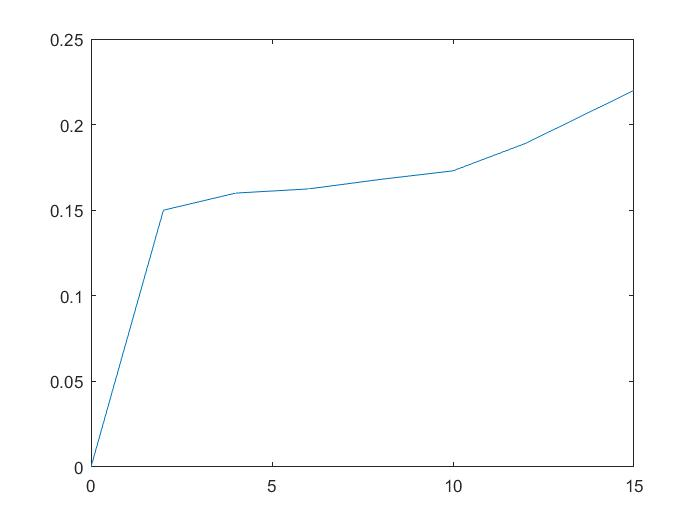
\includegraphics[height=200pt]{2.jpg}
  \item
  Distortion cure with V varying, set U and Y to 1:
  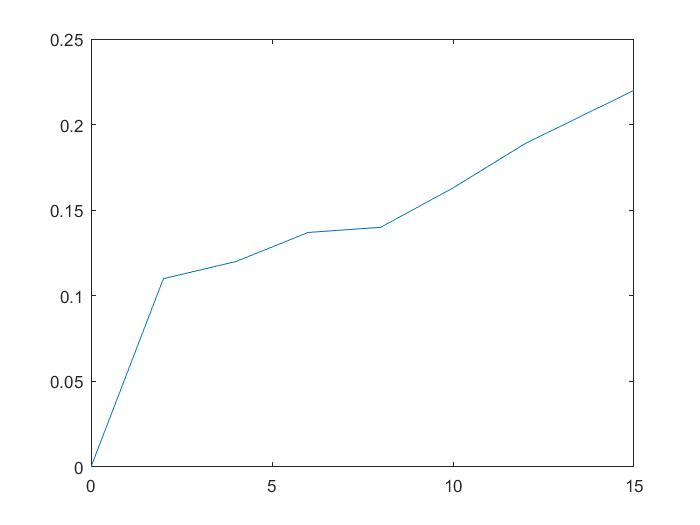
\includegraphics[height=200pt]{3.jpg}
\end{itemize}
	The pattern is that the error rate increases fast, then slow down up to a limit.\\
	First, the average error rates for these three settings are increasing with the sub-sampling factor increasing. Another observation is that Y value is much important compared to the other two values since the error rate increases much faster.\\
  \section*{Q 2}
     The main idea is to subsample differently. For example, instead of sampling with a constant sample interval, for particular image, the histogram is different and the distribution of the texture is  way more different. So, with some calculations like gradient, smaller sample interval is applied to complex part of the image.\\
     Another easier way is to increase the total bits for the image.\\
     Some output results are as followed:\\
     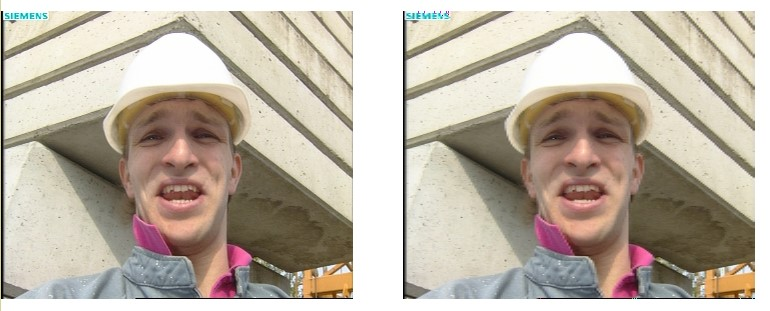
\includegraphics[height=150pt]{4.jpg}
     \\optimized one with Y=4\\
      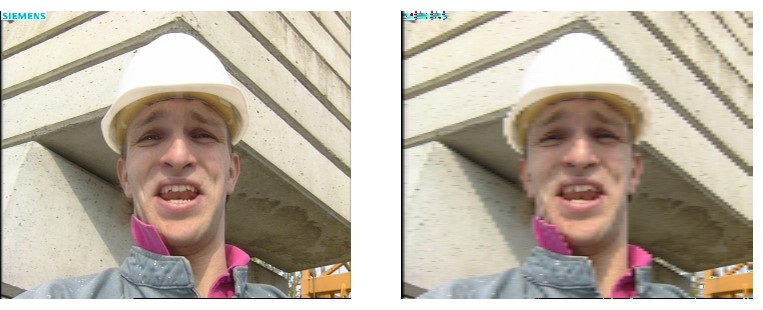
\includegraphics[height=150pt]{5.jpg}
      \\original image with Y=4.
     
\end{document}                          % The required last line
